\begin{figure}[H]
\centering
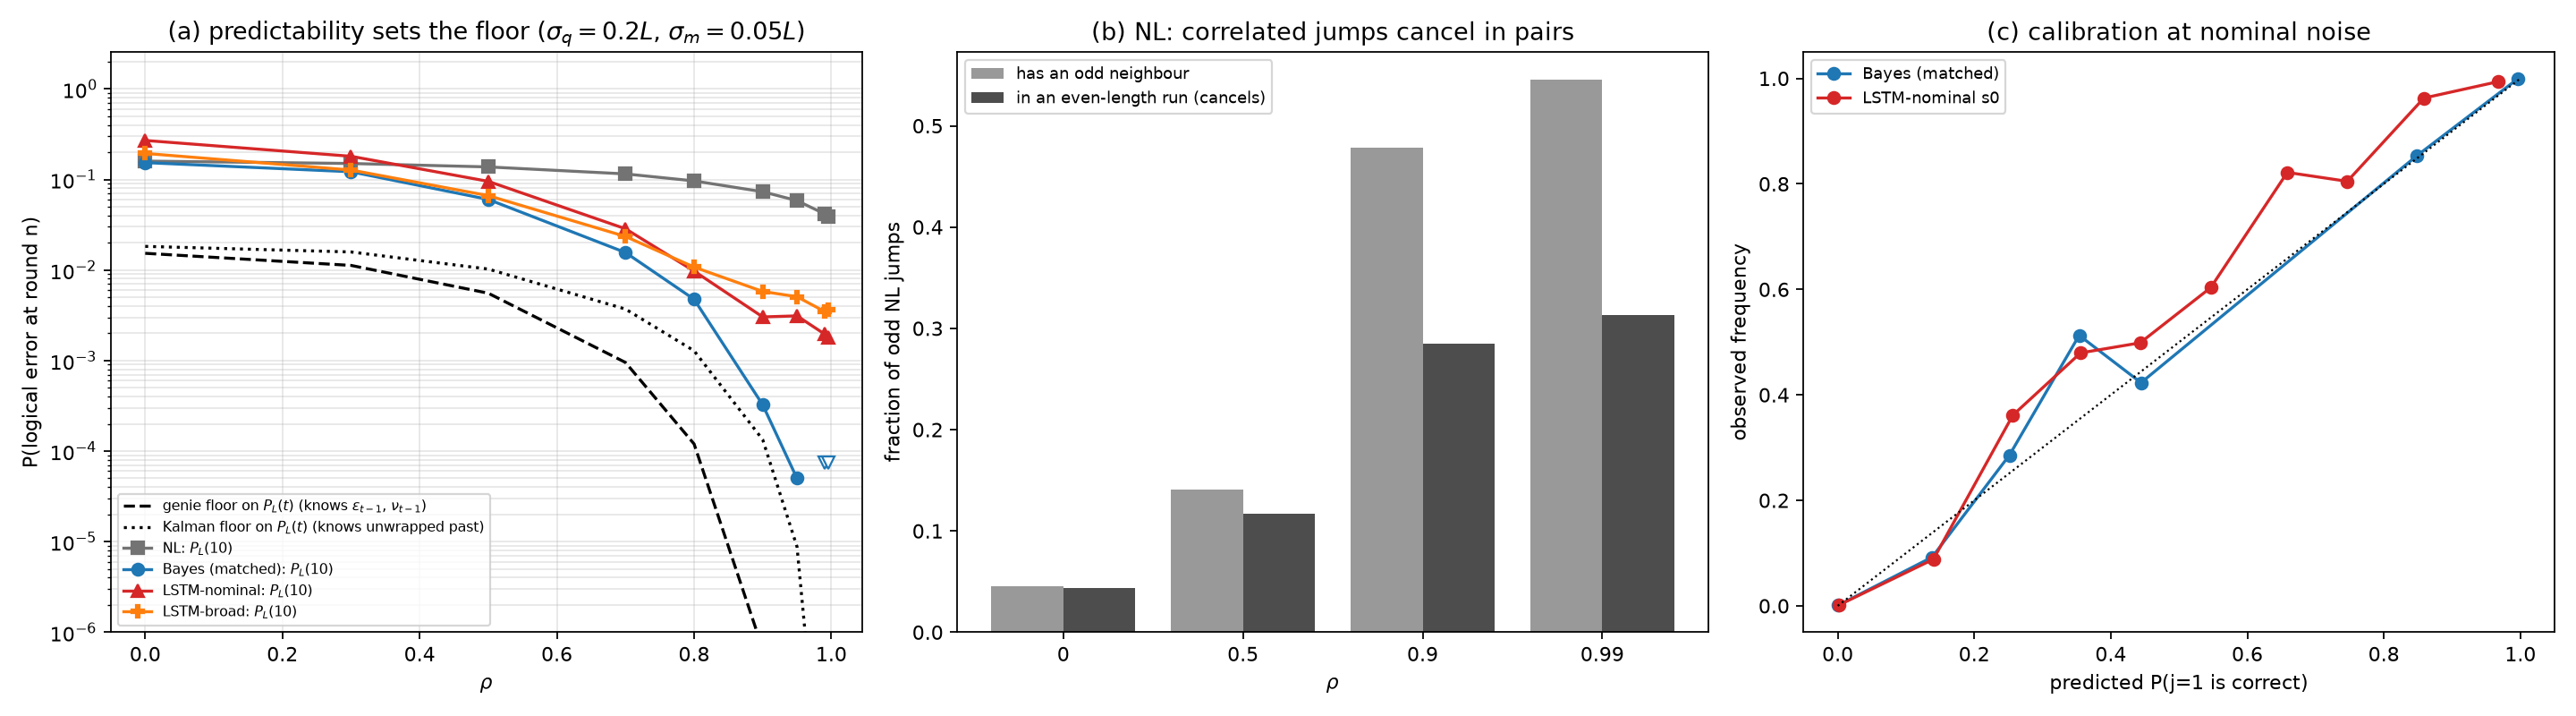
\includegraphics[width=\textwidth]{E8_diagnostics.png}
\caption{E8 diagnostics. (a) $P_L(10)$ against $\rho$ (level~A), with two
analytic floors: a genie that knows $\varepsilon_{t-1}$ and $\nu_{t-1}$, and
the optimal (Kalman) predictor given the \emph{unwrapped} past. (b) NL's odd
jumps cluster as correlation grows. (c) Calibration of the per-round
probability $P(j_t=1\text{ is correct})$ at the nominal point.}
\label{fig:e8}
\end{figure}

\paragraph{Why memory helps: predictability.}
With $c_t=s_t+j_tL$, the only uncertainty in round $t$ is which lattice cell
$z_t=\varepsilon_t+\nu_t-\nu_{t-1}$ fell into~\eqref{eq:z}. The history
predicts $\varepsilon_t$ with an innovation standard deviation of
$\sigma_q\sqrt{1-\rho^2}$, which shrinks from $\sigma_q$ at $\rho=0$ to almost
nothing at $\rho\to1$. Figure~\ref{fig:e8}(a) shows that the per-round floors
follow this.
\begin{itemize}
  \item A decoder that knew the unwrapped past would err in about 1.8\% of
    rounds at $\rho=0$, but only about $10^{-4}$ at $\rho=0.9$.
  \item Matched Bayes tracks this floor at high $\rho$. At $\rho=0.9$ its
    $P_L(10)$ is within a factor of about 3 of the Kalman floor, which knows
    strictly more than the decoder.
  \item At low $\rho$ the gap is wide because errors accumulate over the
    10~rounds.
\end{itemize}

\paragraph{Why NL also improves with $\rho$.}
NL's per-round jump probability does not depend on $\rho$
(\nolinkurl{docs/sim_validation}), yet its $P_L(50)$ falls as $\rho$ grows. The
reason is that correlated jumps come in runs (Figure~\ref{fig:e8}(b)):
\begin{itemize}
  \item at $\rho=0$, \EpairZero{} of odd jumps have an odd neighbour;
  \item at $\rho=0.9$, \EpairNominal{} do, and \EcancelNominal{} sit in
    even-length runs whose parities cancel.
\end{itemize}
This is the same effect reported in the simulator validation.

\paragraph{Why the early rounds zig-zag.}
When $\rho$ is close to 1, a large $\varepsilon$ near $\pm L/2$ is nearly
frozen. The first syndrome cannot tell which cell it is in. If the decoder
guesses wrong, the error then flips the logical state every round until the
evidence (the slow drift of $\varepsilon$) resolves it. This is the odd/even
pattern of Figure~\ref{fig:e1}, and the $\rho\to1$ limit derived in
\texttt{docs/sim\_validation}. Bayes resolves most such cases within a few
rounds. At $\rho\ge0.99$, however, about 1\% of trials have a displacement so
close to the cell boundary that the slow drift never settles it, and those
trials stay wrong after every odd round. That is why $P_L(50)$ (an even round)
vanishes there while the time-averaged error does not.

\paragraph{Why revising decisions matters.}
A decision that looked right given $s_1..s_t$ can be shown wrong by
$s_{t+1},s_{t+2},\dots$ once the drift of $\varepsilon$ becomes visible. The
cumulative rule $J_t=\hat K_t$ undoes such mistakes, while per-round rules
lock them in. The ablations quantify this at the nominal point:
\begin{itemize}
  \item Bayes: $\ErevBayes$ (cumulative) against $\ErevBayesPR$ (per-round);
  \item LSTM: $\ErevLSTM$ against $\ErevLSTMkzero$.
\end{itemize}
In every LSTM, validation selected the cumulative head
(Table~\ref{tab:training}).

\paragraph{Where the LSTM loses to Bayes.}
At the nominal point, the two decoders disagree in only $\EdiagDisagree$ of
trial-rounds. When they disagree, Bayes is right \EdiagBayesRight\% of the
time, and its posterior is almost always decisive there; it is the LSTM's
output that sits close to 0.5. The LSTM's errors are therefore concentrated
in rare rounds that the exact posterior settles clearly but the network has
not learned: rounds with an odd nearest-lattice jump, where these decisions
arise, are only about 2\% of the training data.

This fits the pattern in E2 and E3: the LSTM approaches Bayes where errors
are common (matched LSTM within 2--17\% at $\rho=0.5$ and at
$\sigma_q=0.26L$), and falls behind where they are rare. The LSTM's
probabilities are also biased low (Figure~\ref{fig:e8}(c)). From a predicted
value of about 0.25 upwards, observed frequencies exceed its predicted
$P(j_t=1)$ by up to about 0.15, so it is under-confident above 0.5 and
over-confident towards $j_t=0$ between 0.25 and 0.5. Bayes is approximately
calibrated.

\paragraph{Generalisation over time.}
Run for 200 rounds, all memory decoders keep working well past their
50-round training length (Figure~\ref{fig:e8h}). Errors accumulate slowly:
\begin{itemize}
  \item matched Bayes: $\EhzBayesFifty\to\EhzBayesTwohundred$;
  \item LSTM-nominal: $\EhzLSTMnomFifty\to\EhzLSTMnomTwohundred$;
  \item NL: $\EhzNLFifty\to\EhzNLTwohundred$.
\end{itemize}

\begin{figure}[H]
\centering
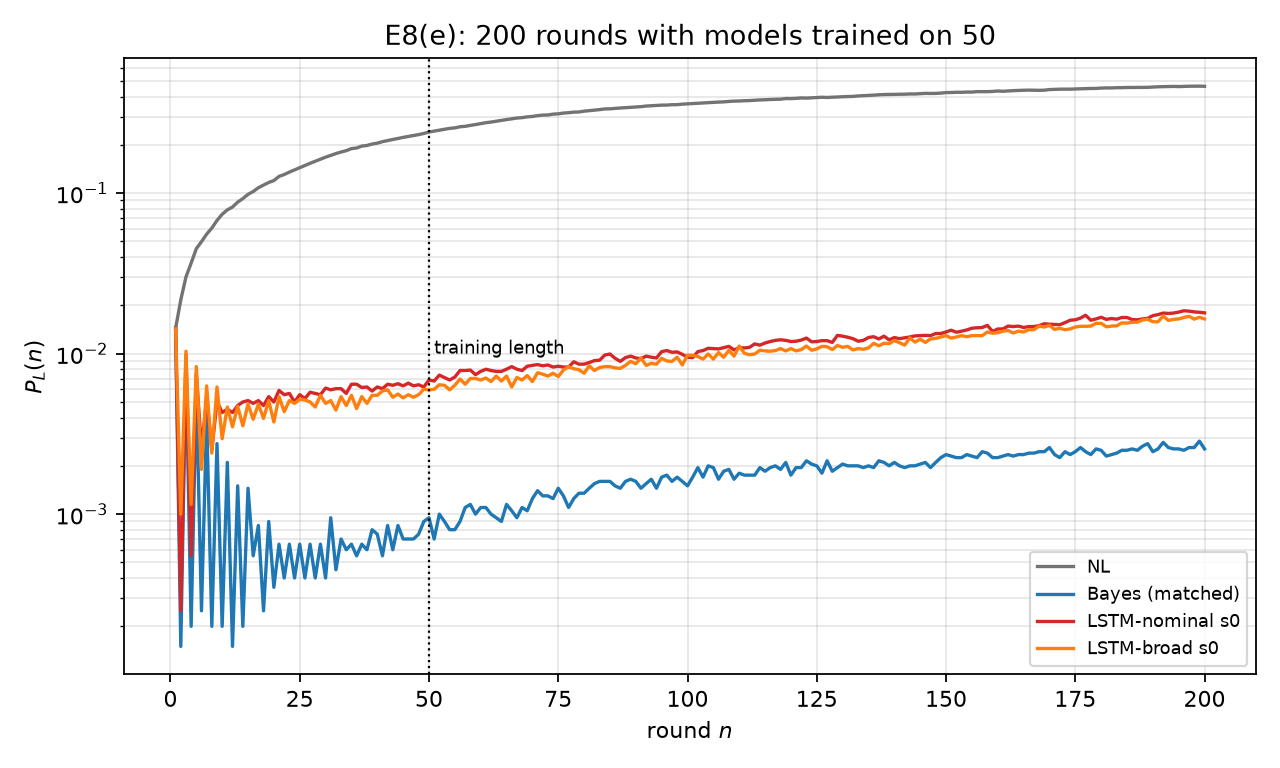
\includegraphics[width=0.62\textwidth]{E8_horizon.png}
\caption{E8(e): 200 rounds at the nominal point; the LSTMs were trained on
50-round sequences.}
\label{fig:e8h}
\end{figure}
